\documentclass[12pt,a4paper]{report}

\usepackage{geometry}
\geometry{left=25mm, right=25mm, top=25mm, bottom=25mm}
\usepackage{setspace}
\setstretch{1.5}
\usepackage{titlesec}
\usepackage{tocloft}
\usepackage{graphicx}
\usepackage{amsmath}
\usepackage{caption}
\usepackage{enumitem}
\usepackage{float}
\usepackage{booktabs}
\usepackage{hyperref}
\usepackage{comment}
\usepackage{natbib}
\usepackage{subcaption}
\usepackage{tikz}
\usetikzlibrary{shapes.geometric}

\title{Automation of nuclear material cladding coating measurement process }
\author{Emma Tekulová }

\titleformat{\chapter}[hang]{\bfseries\LARGE}{\thechapter.}{1em}{}
\titleformat{\section}[hang]{\bfseries\Large}{\thesection}{1em}{}
\titleformat{\subsection}[hang]{\bfseries\large}{\thesubsection}{1em}{}
\titleformat{\subsubsection}[hang]{\bfseries\normalsize}{\thesubsubsection}{1em}{}


\renewcommand{\cftchapfont}{\bfseries}
\renewcommand{\cftsecfont}{\normalfont}
\renewcommand{\cftchappagefont}{\bfseries}
\renewcommand{\cftsecleader}{\cftdotfill{\cftdotsep}}


\usepackage{titlesec}

\usepackage{titlesec}

\titleformat{\chapter}[display]
  {\normalfont\huge\bfseries} 
  {}{0pt}{} 
  \titlespacing*{\chapter}{0pt}{-1cm}{\baselineskip} % Adjust vertical space before the chapter title


\begin{document}

\maketitle
\newpage


\chapter*{Summary}
The data used in this work are from researchers using scanning electron microscope images to investigate the properties of oxidation and coating layers on various materials essential to the nuclear industry. Accurately measuring the thickness of these layers is important for material characterization. The current manual measurement process is time-consuming, and automating it can significantly improve efficiency. Many algorithms can assist with automation, varying widely in complexity and input expectations. While many of these algorithms promise powerful and accurate results, real-world scenarios require substantial groundwork before these tools can be effectively deployed and automation established. This work discusses the challenges and solutions encountered, beginning with the collection and assessment of all available data. It then explores experiments with both conventional computer vision and machine learning algorithms, evaluating their performance. The overall parameters of different solutions are examined, and the most suitable approach is selected. This approach is then seamlessly integrated into the researchers' existing workflow.
\newpage
\chapter*{Souhrn}
Data použitá v této práci pocházejí od výzkumníků, kteří využívají snímky ze skenovacího elektronového mikroskopu ke zkoumání vlastností oxidačních a povlakových vrstev na různých materiálech důležitých pro jaderný průmysl. Přesné měření tloušťky těchto vrstev je klíčové pro charakterizaci materiálů. Současný manuální proces měření je časově náročný a jeho automatizace může výrazně zvýšit efektivitu. Existuje mnoho algoritmů, které mohou pomoci s automatizací, přičemž se liší svojí složitostí a požadavky na vstupní data. Ačkoli mnoho z nich nabízí přesné a výkonné výsledky, v realitě si jejich nasazení vyžaduje rozsáhlou přípravu, aby bylo možné efektivně dosáhnout automatizace. Tato práce se zabývá výzvami a řešeními, které byly při vývoji automatizovaného řešení identifikovány. Začíná sběrem a analýzou dostupných dat, následně se věnuje experimentům s konvenčními algoritmy počítačového vidění a strojového učení, přičemž hodnotí jejich výkonnost. Jsou zhodnoceny parametry různých řešení a vybraný nejvhodnější přístup, který je následně integrován do stávajícího pracovního postupu.
\newpage



\chapter*{Acknowledgements}

    
I would like to express my gratitude to my advisor, \textbf{Ing. Petr Čech, Ph.D.}, and my consultant, \textbf{Mgr. Jaroslav Knotek}, for their guidance and support throughout this work.
\\
The input data used was created with state support from the Technology Agency of the Czech Republic under the THÉTA Program as part of project No. TK04030082 and utilizing the CICRR infrastructure, which is financially supported by the Ministry of Education, Youth, and Sports – project LM2023041.

\newpage

\renewcommand{\contentsname}{\vspace{-1.5cm}Contents}
\addtocontents{toc}{\vspace{-1cm}}
\tableofcontents


\newpage


\chapter{Introduction}

The Research Institute \v{R}e\v{z} conducts numerous projects in the nuclear industry. Some of these involve electron microscopy and the analysis of materials subjected to high temperatures and aggressive environments, such as those found in nuclear reactors. A significant portion of these projects requires extensive manual image analysis, making automation a crucial challenge. Currently, image analysis is performed using various processing tools, including Fiji~\cite{Schindelin2012} by ImageJ. This thesis aims to automate one of these manual processes.

The primary focus of this work is the segmentation of coating layers in material samples. These images contain both coating and oxidation layers, with coating layers exhibiting greater uniformity, whereas oxidation layers present irregular structures, as illustrated in Figure~\ref{fig:coating-oxidation}. By initially addressing the segmentation of coating layers, this thesis evaluates the potential of automation in reducing analysis time while maintaining sufficient accuracy. If successful, future work could extend this approach to more complex cases, such as samples without coating layers and those with multiple oxidation types.

Three computer vision algorithms are explored to achieve segmentation, ranging from traditional clustering techniques to advanced deep-learning models. The first method explored is K-means clustering, an unsupervised algorithm that does not require labeled data. While K-means provides a lightweight approach, its effectiveness is hindered by the non-homogeneous nature of coating layers. Due to variations in layers, colors, and structures, different parameter settings must be adjusted for each image, limiting its practical usability. Further details on this method are discussed in Section~\ref{sec:kmeans}.

The second approach involves Convolutional Neural Networks (CNNs), which, unlike K-means, require labeled data and are computationally more demanding. However, CNNs offer good segmentation accuracy once trained. This thesis examines three levels of label precision, balancing annotation effort with segmentation performance. The original labeling come in the form of information about the thinkers of the coating layer at 10 places per picture. From this can be easily reconstructed polygon labels which are not that precise. On the other hand the creation of more precise labels requires extra time of the scientist on top of clacical labeling ith 10 lines. Although the most precise labels yield the best results, less precise labels provide comparable outcomes while significantly reducing annotation time, as discussed in Section~\ref{sec:cnn}.

A major limitation of CNN-based methods is the computational cost of prediction. The available hardware lacks sufficient memory for complex image processing, leading to slow predictions, particularly when relying on CPU computation. Under the current setup, a single prediction requires approximately 14 seconds, compared to around one minute for manual segmentation. Thus, the trade-off between segmentation accuracy and computational efficiency remains a key consideration.

The "Segment Anything" (SAM) model \cite{kirillov2023segany} represents a state-of-the-art approach in image segmentation, leveraging transformers. While SAM holds significant potential to improve segmentation performance, it comes with considerably higher computational demands due to its robustness and the large number of parameters involved. Specifically, the number of parameters in the SAM model and U-Net in this thesis was measured, with the SAM model containing over 21 times more parameters than U-Net. This substantial increase in model complexity leads to a corresponding rise in hardware requirements during predictions. Consequently, the computational demands of the SAM model exceed the capabilities of the available hardware, particularly in the absence of GPU infrastructure. As a result, fine-tuning and evaluating the SAM model was not pursued in this thesis. However, as hardware resources continue to improve, this approach may become a viable option for future research.

In the following chapters, the thesis will focus on the use of K-Means clustering and label creation to develop a cohesive dataset for CNNs with U-Net architecture. It will also address the training and optimization of the model's hyperparameters. Ultimately, the best-performing model will be integrated into the research workflow, and the results obtained by the researcher using this model will be evaluated.



 % the SAM model contains approximately 641 million parameters (measured in jupyter notebook, but on site they say it is 632M for the initial first image encoder https://segment-anything.com/), which is over 21 times more than the 29.9 million parameters in the U-Net model used in this thesis. I tried it with https://stackoverflow.com/questions/49201236/check-the-total-number-of-parameters-in-a-pytorch-model

\begin{figure}[H]
    \centering
    \begin{subfigure}{0.40\textwidth}
        \centering
        \includegraphics[width=\linewidth]{PICTURES/intro/115.png}
        \caption{Material sample with coating.}
        \label{fig:coating}
    \end{subfigure}
    \hfill
    \begin{subfigure}{0.40\textwidth}
        \centering
        \includegraphics[width=\linewidth]{PICTURES/intro/625_3500h_low_cross_strana1_13.png}
        \caption{Material sample with oxidation.}
        \label{fig:oxidation}
    \end{subfigure}
    \caption{Coating and oxidation layers in the material sample.}
    \label{fig:coating-oxidation}
\end{figure}




\chapter{Practical Part}
\section{Data}

The dataset consists of images captured using a scanning electron microscope (SEM). These images are part of a study focused on the thickness of coating cladding layers applied to various materials, both before and after being subjected to high temperatures and aggressive environments, to assess the properties of these layers. The layers of interest are marked within red rectangular boxes in Figure~\ref{fig:three-images}. These layers exhibit varied characteristics, such as differences in color, number of layers, and degrees of damage.

\begin{figure}[ht]
    \centering
    \begin{subfigure}{0.3\textwidth}
        \centering
        \includegraphics[width=\linewidth]{PICTURES/original_data/11.png}
        \label{fig:subfig1}
    \end{subfigure}
    \hfill
    \begin{subfigure}{0.3\textwidth}
        \centering
        \includegraphics[width=\linewidth]{PICTURES/original_data/177.png}
        \label{fig:subfig2}
    \end{subfigure}
    \hfill
    \begin{subfigure}{0.3\textwidth}
        \centering
        \includegraphics[width=\linewidth]{PICTURES/original_data/208.png}
        \label{fig:subfig3}
    \end{subfigure}
    \caption{SEM images with highlighted coating layers in red boxes.}
    \label{fig:three-images}
\end{figure}

\subsection{Manual Data Processing}\label{sec:ManualProc}

The images are initially obtained in *.tif format after the measurements with the SEM. Then they are processed using Fiji, an open-source image processing software that is a distribution of ImageJ \cite{Schindelin2012}. A predefined template consisting of 20 lines is used for measurements, each corresponding to a specific measurement region. The first ten lines, indexed 1 to 10, are employed to measure the thickness of the coating layer, while the second set of ten lines, located beneath the first, are used to measure oxidation. The lines are evenly distributed across the image's width and share a constant x-coordinate.

Subsequent to the initial measurements, each of the 20 lines is manually adjusted to align with either the oxidation or the coating layer. After all adjustments are completed, the measurements are exported to Excel for statistical analysis. If a layer is absent at the location of a predefined line, the line is left in its position but is later marked as 0.0 in the corresponding Excel spreadsheet. 

The images are grouped into batches of approximately 30, with each batch containing images of the same material, though different parts of the material are captured in each image, leading to a high degree of similarity among the images in each batch. The initial image of each batch typically takes longer to process since the line adjustments from the previous image are reused for the other images in the same batch. As the remaining images within a batch are more similar, they require less time for adjustment. The primary challenges arise in images where significant oxidation is present, which may destroy the coating layer.

Figure~\ref{fig:Fiji} illustrates the measurements performed in Fiji. Lines 1 to 10, used for measuring the coating layer, are shown. In this example, no oxidation layer is present.

\begin{figure}[H]
    \centering
    \includegraphics[width=0.7\linewidth]{PICTURES/625_Al2O3_3500h_low_cross_strana2_13_measurements.png}
    \caption{Measurement in Fiji software.}
    \label{fig:Fiji}
\end{figure}

\newpage
Although oxidation and coating layers are both critical for material characterization, this thesis focuses specifically on automating the measurement of coating layer thickness in SEM images. Coating layers prevent underlying materials from oxidizing, making oxidation layers less common in samples that feature coatings.


\subsection{Fiji Adjustments}\label{sec:1.2.2}

The first modification involved the customization of the `StartUpMacro` in Fiji, which runs automatically each time the program is launched. Three new buttons were incorporated into the interface: one for saving measurements, another for adjusting the scale, and a third for displaying the default lines.

The \texttt{Save Measurement} button was implemented to store data from the 20 lines required to create the dataset necessary for automation. This feature ensures that the required measurements are automatically saved.

The \texttt{Adjust Scale} button was added to streamline user interaction with Fiji, addressing the need to manually adjust the scale at the start of each session. Since the scale, visible at the bottom of the image, remains constant across all images, this functionality simplifies the process.

The \texttt{Set Default ROI} button was introduced to allow the researcher to quickly access the prepared default 20 lines for new batch.

Furthermore, the extraction of the final measured lengths into an Excel file was simplified.

\subsection{Dataset}

As previously mentioned, the first step in dataset creation was gathering data. Prior to this, results were stored exclusively in Excel tables, which included the lengths of the measurement lines but lacked positional information, rendering them insufficient for generating a comprehensive dataset. After collecting enough data thanks to the Fiji adjustments~\ref{sec:1.2.2}, stored in a zip folder containing 20 *.roi files (each representing one measurement line), the dataset was created.

\subsubsection{Polygon Labels}

The initial set of labels was generated using measured data from ten measurement lines. The upper ten points of each line were connected to form a boundary curve, and the same process was applied to the lower points. The space between these two curves was then filled to generate the mask. However, due to missing information at the edges of the image, cropping of both the images and the masks was needed. Figures~\ref{fig:polygon_sem_color} and~\ref{fig:polygon_sem} illustrate that the masks do not extend to the edges of the images.

This labeling process was automated using a Python script. The script loads each image along with the corresponding zip folder containing the line measurements. The x and y coordinates of these lines are stored in arrays, which are then mapped onto an Excel sheet. Any lines marked as missing (labeled as 0) in Excel are excluded, even if they are present in the folder.

To interpolate the boundary points, cubic spline interpolation \cite{fritsch1980monotone} was employed. The upper and lower boundary points, stored in arrays, were used to create a spline model, which was then applied to generate the boundary curve. The interpolation function was used with a smoothing parameter of s=0 to ensure that the interpolation closely followed the measured points. The space between the curves was filled, resulting in a binary mask. The mask was resized to match the original image dimensions and saved as a binary mask.

This approach enabled the automated generation of masks from the measured oxidation lines, ensuring that the labels were consistent with the scientific data.



\subsubsection{K-means Labels} \label{sec:kmeans}

The K-means algorithm \cite{lloyd1982least} is a clustering method used in unsupervised machine learning, designed to minimize a function that measures the quality of cluster formation. The algorithm selects $k$ random points as cluster centers from the dataset, assigning each data point to the nearest center based on distance. The geometric center of each cluster is then recalculated, and the process repeats until a convergence criterion is met.

K-means is particularly effective for images with distinct pixel colors. One of the key advantages of K-means is that it does not require prior labels, but the value of $k$ (the number of clusters) must be chosen carefully. Thus, the optimal $k$ was determined through testing for each batch of images.

In most cases, further processing was necessary, particularly to isolate the coating layer while eliminating noise. As illustrated in Figures~\ref{fig:kmean_sem_color} and~\ref{fig:kmean_sem}, K-means encountered difficulty distinguishing between oxidation and the coating layer, as their pixel values were similar and even formed a continuous cluster. Consequently, the algorithm alone was insufficient for accurately measuring the coating layer.

\subsubsection{K-means Refined}

To improve the accuracy of the K-means labels, the entire dataset was reviewed collaboratively with the researcher, and the masks were manually refined using image editing software. These manually refined masks, considered the most accurate, were validated by the researcher. The final version of the masks was then used as a test dataset for further automation.


\begin{figure}[ht]
    \centering
    \begin{subfigure}{0.3\textwidth}
        \centering
        \includegraphics[width=\linewidth]{PICTURES/MASK/POLYGON316L_W_3500h_low_cross_strana1_07.png}
        \caption{Polygon mask}
        \label{fig:polygon_sem_color}
    \end{subfigure}
    \hfill
    \begin{subfigure}{0.3\textwidth}
        \centering
        \includegraphics[width=\linewidth]{PICTURES/MASK/KMEAN316L_W_3500h_low_cross_strana1_07.png}
        \caption{K-Means mask}
        \label{fig:kmean_sem_color}
    \end{subfigure}
    \hfill
    \begin{subfigure}{0.3\textwidth}
        \centering
        \includegraphics[width=\linewidth]{PICTURES/MASK/149_original.png}
        \caption{Refined K-Means}
        \label{fig:kmean_refined_color}
    \end{subfigure}
    \caption{Masks on SEM image}
    \label{fig:three-masks_color}
\end{figure}

\begin{figure}[ht]
    \centering
    \begin{subfigure}{0.3\textwidth}
        \centering
        \includegraphics[width=\linewidth]{PICTURES/MASK/316L_W_3500h_low_cross_strana1_07(2).png}
        \caption{Polygon mask}
        \label{fig:polygon_sem}
    \end{subfigure}
    \hfill
    \begin{subfigure}{0.3\textwidth}
        \centering
        \includegraphics[width=\linewidth]{PICTURES/MASK/316L_W_3500h_low_cross_strana1_07.png}
        \caption{K-Means mask}
        \label{fig:kmean_sem}
    \end{subfigure}
    \hfill
    \begin{subfigure}{0.3\textwidth}
        \centering
        \includegraphics[width=\linewidth]{PICTURES/MASK/316L_W_3500h_low_cross_strana1_07(1).png}
        \caption{Refined K-Means}
        \label{fig:kmean_refined_sem}
    \end{subfigure}
    \caption{Binary masks}
    \label{fig:three-masks}
\end{figure}

\include{03_CNN}
\include{04_integ_time}
\include{05_SAM}


\chapter{Conclusion}

This thesis successfully addresses the challenge of automating a time-consuming manual process in the nuclear industry. Researchers are often required to perform repetitive, labor-intensive measurements. The primary goal was to develop a solution that integrates seamlessly into the researcher’s workflow without causing disruptions. The thesis focused on a specific category of coating-layer images with relatively homogeneous properties, in contrast to other images in the dataset. It was shown that segmentation of more complex, heterogeneous images is a viable direction for future work.

Three approaches were evaluated. First, the classical K-means algorithm was found to be computationally efficient, but it lacked universal applicability due to the variability of coating layers. This made it unsuitable for a streamlined workflow without extensive post-processing. Second, the Segment Anything Model (SAM) was considered, but hardware limitations made it infeasible for the given problem. Finally, Convolutional Neural Networks (CNNs) were explored. This solution required labeled data. Three types of labels were developed. The model was trained on the most precise set, but it was found that even the least manually intensive labels were effective for training, despite being less accurate. This insight suggests that efficient model retraining is also possible with this kind of labels and that the model could be adapted to handle more complex images in the future.

The optimization and testing of the model were thoroughly discussed, with results measured using the Intersection over Union (IoU) metric. The model achieved a mean IoU of 95.47\%, demonstrating its high accuracy in segmenting coating layers.

After integrating the model into the researcher’s workflow, the practical impact was clear. The time required for measurement tasks was reduced by half. For images similar to the training dataset, over 90\% of predicted measurements required no further manual adjustments. However, for images from batches with significantly different characteristics, performance declined, highlighting the need for further re-training.

With the code infrastructure in place, future improvements can focus on streamlining the training process and enhancing prediction accuracy. The current model was trained on fewer than 100 images from a limited number of batches, which is insufficient for creating a fully robust model. Nevertheless, even when incorrect, the model's average deviation was approximately five pixels, resulting in substantial time savings. This efficiency will accelerate the generation of additional labeled data, creating a feedback loop for continuous improvement. The iterative workflow is illustrated in figure~\ref{fig:workflow-diagram}.

\begin{figure}[H]
    \centering
    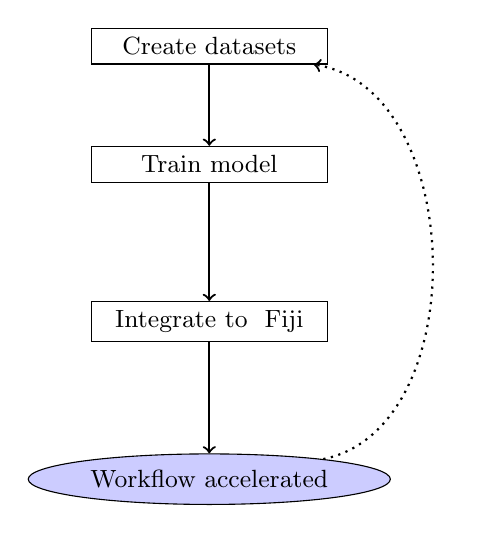
\begin{tikzpicture}[node distance=1.5cm, every node/.style={align=center, font=\small}]

        \node[rectangle, draw, minimum width=3cm] (dataset) {Create datasets};
        \node[rectangle, draw, minimum width=3cm, below of=dataset, yshift=0cm] (train) {Train model};
        \node[rectangle, draw, minimum width=3cm, below of=train, yshift=-0.5cm] (integration) {Integrate to \ Fiji};
        \node[ellipse, draw, fill=blue!20, minimum width=3cm, below of=integration, yshift=-0.5cm] (result) {Workflow accelerated};

        % Arrows
        \draw[->, thick] (dataset) -- (train);
        \draw[->, thick] (train) -- (integration);
        \draw[->, thick] (integration) -- (result);
        \draw[->, thick, dotted] (result) to[bend right=80] (dataset);
    \end{tikzpicture}
    \caption{Workflow of model integration and performance improvement.}
    \label{fig:workflow-diagram}
\end{figure}

In conclusion, this thesis automates a portion of the researcher’s measurement process and establishes a pipeline for continuous model retraining and improvement. It also demonstrates that polygon masks, generated directly from researcher annotations, are sufficient for training segmentation models. These results suggest that similar models can be developed for other types of images within the researcher’s domain. The improvements brought by this work will lead to time savings and improved efficiency. This work highlights the practical impact of deep learning in automating image analysis tasks in the nuclear industry.

\chapter{Appendix}

The complete implementation of this thesis, including preprocessing, label generation, model training, and evaluation scripts, is available at [GitHub Repository Link (will be added in future when it has documentation, proper README,...)].

This project benefited from various open-source libraries that facilitated image processing, deep learning model training, and evaluation. A detailed list of dependencies and libraries used can be found in the repository’s requirements.txt file.

Additionally, this text was refined and grammar-checked using ChatGPT \cite{chatgpt2025}, and Grammarly \cite{grammarly2025}.


\bibliographystyle{plain}
\bibliography{CNN}


\newpage
\listoffigures
\newpage

\listoftables
\newpage

\chapter*{List of Abbreviations}
\begin{itemize}
    \item \textbf{TP} - True Positive
    \item \textbf{TN} - True Negative
    \item \textbf{FP} - False Positive
    \item \textbf{FN} - False Negative
    \item \textbf{CNN} - Convolutional Neural Network
    \item \textbf{LR} - Learning Rate
    \item \textbf{LRS} - Learning Rate Scheduler
    \item \textbf{SEM} - Scanning electron microscope
    \item \textbf{IoU} - Intersection over union
    %\item \textbf{ROI} - Region of interest (here, measurement lines)
    \item \textbf{SAM} - Segment Anything Model
\end{itemize}




\end{document}
